\documentclass{article}
\usepackage{iclr2026_conference,times}

\usepackage{booktabs}
\usepackage{graphicx}
\usepackage{xcolor}
\usepackage{microtype}
\usepackage{amsmath}
\usepackage{enumitem}
\usepackage{url}

% Non-anonymous preprint: keep the ICLR author block rather than the
% double-blind placeholder, but do not claim acceptance in the header.
\iclrfinalcopy
\lhead{Preprint --- technical note, August 2026}

\definecolor{phcolor}{RGB}{192,64,0}
\newcommand{\PH}[1]{\textcolor{phcolor}{\texttt{\{\{\detokenize{#1}\}\}}}}

\setlength{\bibsep}{3pt plus 0.5ex}
\def\bibfont{\small}
% Float placement: keep at least a third of every page for text, so page
% breaks do not land mid-sentence behind a table.
\renewcommand{\topfraction}{0.72}
\renewcommand{\textfraction}{0.28}
\renewcommand{\floatpagefraction}{0.7}

\title{The Price of a Mismatched Tokenizer:\\ Distribution Shift as an Efficiency Tax}
\author{Guy Kaplan \\
\normalfont August 2026}

\begin{document}
\maketitle

\begin{abstract}
\noindent A tokenizer is trained once, on one corpus, and then deployed on whatever traffic arrives. We ask what that mismatch costs. Coding theory predicts that the number of tokens a text costs grows with the divergence between the deployment distribution and the tokenizer's training distribution. We confirm this across five target corpora, from English chat to Turkish Wikipedia: token inflation is proportional to divergence, with a slope near unity. Language whose script the vocabulary does not cover breaks this law, and we show by controlled substitution that the break is a coverage failure rather than a measurement artifact. A second cost runs alongside the first, as unused vocabulary entries consume parameters and output-layer compute at every decoded token. Both costs are cheap to measure and largely refundable: extending a deployed vocabulary recovers most of the gap for a fraction of a percent of model parameters.
\end{abstract}

\section{A tokenizer is a code}
\label{sec:setup}

Every token a language model reads is one it must attend over, cache, and bill for, and how many tokens a text costs is settled before the model runs, by a tokenizer fitted to somebody else's corpus. We argue that this makes a mismatched tokenizer a standing tax on compute, latency, and context rather than a preprocessing detail, and we show that the tax is predictable from a single number. This section derives two forms of it, \S\ref{sec:lit} calibrates them against published measurements, and \S\ref{sec:demo} tests them on six corpora.

A subword tokenizer \emph{is} a code in the information-theoretic sense \citep{zouhar2023tokenization}. A vocabulary trained on a corpus distribution $P$ acts as an approximately lossless code whose expected code length is near-optimal for $P$. Deployed on traffic from a different distribution $Q$, it pays the classical penalty for coding one source with another's code: expected code length rises from $H(Q)$ to roughly $H(Q) + D_{\mathrm{KL}}(Q\,\|\,P)$ bits per byte. Per-token information content varies only within a limited range at fixed vocabulary size, which is the quantity R\'enyi efficiency measures \citep{zouhar2023tokenization}, so those extra bits must largely surface as extra tokens. Writing $L$ for the \emph{token inflation}, the ratio of token counts under the mismatched and matched tokenizers minus one, we get
\begin{equation}
L \;\approx\; \frac{D_{\mathrm{KL}}(Q\,\|\,P)}{H(Q)}.
\label{eq:inflation}
\end{equation}

Two caveats bound this. BPE is a greedy merge procedure rather than an optimal code, and bits per token is only approximately constant, so we claim a slope near unity with scatter, not a functional form. Compression is also not everything, since tokenizers of equal compression can differ in downstream quality \citep{schmidt2024tokenization}; $L$ prices efficiency, not capability.

The same cost has a second reading through vocabulary coverage. If a fraction $(1-\rho)$ of $Q$'s token occurrence mass is uncovered by the vocabulary and splits into $s$ pieces on average, each affected token contributes $s-1$ extra tokens, giving $L \approx (s-1)(1-\rho)$. The two readings agree while coverage holds. When coverage collapses, which in practice means a change of script, the second becomes a distinct regime that a smooth divergence estimate cannot see, and \S\ref{sec:demo} exhibits both.\footnote{Arithmetic for every quantity marked as derived in this note is given step by step in \texttt{derivations.md} in the accompanying repository.}

\section{What the literature already measures}
\label{sec:lit}

The tax has been measured piecewise, but never against an explicit divergence axis, which is the gap this note addresses. The standard metric is \emph{fertility}, the average number of subwords per tokenized word, and higher fertility on a given language correlates with worse monolingual performance for multilingual models \citep{rust2021tokenizer}. \citet{gowda2020finding} showed that vocabulary size itself has an optimum in machine translation: too small a vocabulary inflates sequences, too large a one leaves its units undertrained. The mismatch therefore has two knobs, and both are billed for.

Arranged by divergence regime, published measurements form a consistent staircase (Table~\ref{tab:calibration}). Adjacent English domains cost percent-level inflation, while specialist domains cost tens of percent. For code the effect is documented in reverse: \citet{dagan2024tokenizer} report that a code-aware tokenizer compresses code by more than 40\% relative to the Llama tokenizer, which inverts to roughly 67\% inflation when a natural-language tokenizer meets code. Across related European languages fertility ratios of 1.5--2$\times$ are typical, and at the extreme \citet{petrov2023language} find encodings up to 15$\times$ longer than English, where byte fallback dominates and the tax turns multiplicative. The middle rows matter most in practice, covering specialist domains, code, and neighbouring languages, and they are the least systematically measured.

%TC:ignore
\begin{table}[t]
\centering
\small
\begin{tabular}{@{}p{4.2cm}p{2.1cm}p{1.9cm}p{4.2cm}@{}}
\toprule
Shift ($P \to Q$) & Divergence (bits/byte, est.) & Inflation & Source \\
\midrule
Web English $\to$ news English & $<0.05$ & 1--3\% & (est.) \\
English $\to$ biomedical/legal & 0.1--0.3 & 10--25\% & domain-vocab studies (est.) \\
NL tokenizer $\to$ source code & 0.3--0.6 & $\approx$33--67\% & \citep{dagan2024tokenizer}, inverted \\
English $\to$ related European & 0.5--1 & 1.5--2$\times$ & \citep{petrov2023language} \\
English $\to$ morphology-rich & 1--2 & 2--4$\times$ & \citep{petrov2023language,rust2021tokenizer} \\
English $\to$ byte-fallback script & $\gg 2$ & up to 15$\times$ & \citep{petrov2023language} \\
\bottomrule
\end{tabular}
\caption{Published inflation measurements arranged by estimated divergence regime. The divergence column organizes the rows; it is not itself a measurement.}
\label{tab:calibration}
\end{table}
%TC:endignore

\section{Where the tax lands}
\label{sec:propagation}

Having priced the mismatch in tokens, we now trace where those tokens are charged. Inflation does not stay in the tokenizer: it propagates undiminished into every quantity a deployment budgets for, linearly in most and quadratically in attention (Table~\ref{tab:propagation}). At 30\% inflation, which sits between the specialist-domain and code regimes of Table~\ref{tab:calibration}, a user pays a third more for the same answer, waits a third longer for it, and runs out of context a quarter sooner, for no reason visible anywhere in the model.

%TC:ignore
\begin{table}[t]
\centering
\small
\begin{tabular}{@{}lll@{}}
\toprule
Quantity & Scales as & At $L = 0.3$ \\
\midrule
Decode latency, API cost, KV-cache & $(1+L)$ & $\times 1.30$ \\
Effective context window & $1/(1+L)$ & $-23\%$ \\
Attention FLOPs & $(1+L)^2$ & $\times 1.69$ \\
\bottomrule
\end{tabular}
\caption{Propagation of token inflation $L$ (derived). A Llama-3.1-8B KV cache holds 128\,KiB per token, so an 8k-token conversation at $L = 0.3$ carries roughly 322\,MB of extra cache.}
\label{tab:propagation}
\end{table}
%TC:endignore

A second tax runs alongside the first. We call it \emph{dead vocabulary}: entries a deployment pays for in parameters and in output-layer compute at every decoded token, and never uses. Writing $V$ for vocabulary size, $d$ for hidden width, and $f$ for the fraction of the vocabulary that receives approximately no mass under $Q$,
\begin{equation}
\begin{aligned}
\text{wasted head compute} \;&\approx\; \frac{f\,V d}{N_{\text{non-emb}}}
\quad\text{per decoded token,}\\[2pt]
\text{wasted parameters} \;&\approx\;
\begin{cases}
f \cdot 2Vd & \text{untied},\\
f \cdot Vd & \text{tied}.
\end{cases}
\end{aligned}
\label{eq:deadvocab}
\end{equation}
We follow the non-embedding-parameter convention of \citet{kaplan2020scaling}, and vocabulary FLOPs are dominated by the output matmul \citep{tao2024scaling}. Table~\ref{tab:headshare} instantiates this on three public configurations. The tax falls hardest on small models with wide vocabularies, where the output layer is roughly a fifth of per-token compute, and it vanishes at 70B scale. Trimming recovers the waste: \citet{abdaoui2020load} cut up to 45\% of multilingual BERT's parameters with comparable accuracy, and modern trimming pipelines report the same \citep{ushio2023trimming}. Oversized vocabularies also carry a quality cost, since rarely-seen entries stay undertrained \citep{land2024fishing}.\footnote{Training amplifies the space cost, since the logits tensor is $B \times T \times V$: one 8{,}192-token sequence at $V = 128{,}256$ in fp32 occupies about 4.2\,GB (derived).}

%TC:ignore
\begin{table}[t]
\centering
\small
\begin{tabular}{@{}lrrrr@{}}
\toprule
Model & $V$ & $d$ & $Vd/N_{\text{non-emb}}$ & Output-layer share of compute \\
\midrule
Gemma-2-2B (tied) & 256{,}000 & 2{,}304 & 29.1\% & 22.6\% \\
Llama-3.1-8B & 128{,}256 & 4{,}096 & 7.5\% & 7.0\% \\
Llama-3.1-70B & 128{,}256 & 8{,}192 & 1.5\% & 1.5\% \\
\bottomrule
\end{tabular}
\caption{Embedding and output-layer shares, derived from public configurations. A dead fraction $f$ wastes $f$ times the last column.}
\label{tab:headshare}
\end{table}
%TC:endignore

The two taxes compose. Against a matched-tokenizer, right-sized-vocabulary baseline, the total overhead is
\[
\frac{\mathrm{cost}(Q)}{\mathrm{cost}_{\mathrm{opt}}(Q)} \;\approx\; \Bigl(1+\tfrac{D_{\mathrm{KL}}}{H}\Bigr)\Bigl(1+\tfrac{f\,Vd}{N_{\text{non-emb}}}\Bigr),
\]
to first order in $f\,Vd/N$. We call this product the \emph{mismatch tax}. Its two factors co-vary, since both grow with the shift, and \S\ref{sec:demo} measures that co-variation directly. On the small configuration, a specialist deployment with 30\% inflation and half its vocabulary dead pays about 49\% overhead (derived). To our knowledge the two factors have been quantified only separately, never as a product.

\section{Measuring the tax on six corpora}
\label{sec:demo}

We now test Eq.~\eqref{eq:inflation} directly. The deployed tokenizer is GPT-2's, with an OpenWebText sample standing in for its training distribution $P$. The targets $Q$ are Hebrew and Turkish Wikipedia, Python source, PubMed abstracts, and English chat, each 30--40\,MB, with all measurement on held-out splits.\footnote{Chat (OpenAssistant) supplied 33.6\,MB, and a short-line filter removes 29\% of code lines, so the Python corpus is gappy rather than runnable.} For each corpus we measure four quantities:

\begin{enumerate}[leftmargin=2em,itemsep=1pt,topsep=3pt]
\item \textbf{Inflation $L$}, from the bytes per token of the deployed tokenizer against a BPE tokenizer retrained on $Q$ at \emph{equal} vocabulary size. Comparing two tokenizers on identical text makes $L$ immune to the mean-word-length confound that makes bytes per token incomparable across corpora.
\item \textbf{Divergence} $D_{\mathrm{norm}} = \bigl(H_{\times}(Q,P) - H(Q)\bigr)/H(Q)$, from interpolated byte $n$-gram models. Both terms are held-out cross-entropies biased upward by the model order, so $D_{\mathrm{norm}}$ tracks $D_{\mathrm{KL}}(Q\,\|\,P)/H(Q)$ rather than estimating it exactly.
\item \textbf{Coverage} under $Q$: the dead fraction $f$ of Eq.~\eqref{eq:deadvocab}, and the effective vocabulary $V_{\mathrm{eff}}$, the perplexity of the token unigram distribution.
\item \textbf{Recovery}, the share of the deployed-to-retrained gap closed by appending target-domain merges to the deployed vocabulary.
\end{enumerate}

%TC:ignore
\begin{figure}[!t]
\centering
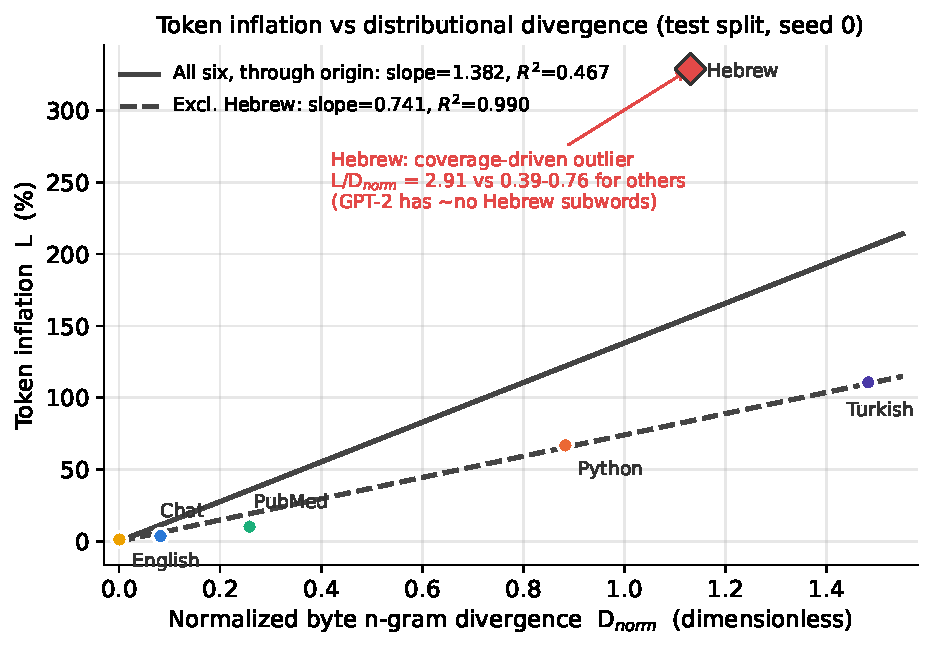
\includegraphics[width=0.72\linewidth]{figures/fig1_inflation_vs_divergence.pdf}
\caption{Token inflation against divergence, one point per corpus. Excluding the coverage-driven Hebrew outlier, the through-origin fit has slope 0.741 and $R^2 = 0.990$; Eq.~\eqref{eq:inflation} predicts a slope near 1.}
\label{fig:slope}
\end{figure}
%TC:endignore

Inflation tracks divergence closely wherever the script is covered. Five of the six corpora fall on a line through the origin, with a slope of $0.741$ and $R^2 = 0.990$ (Figure~\ref{fig:slope}). The fit leans on no one of them: leaving each corpus out in turn keeps the slope between $0.726$ and $0.749$, Turkish included. Fitting all six instead drops $R^2$ to $0.47$, and the same leave-one-out test then swings the slope by nearly a factor of three. The two fits differ in kind of stability rather than in fit quality, and Hebrew alone accounts for the difference.

Hebrew marks the second regime, and its cost is not that its divergence is large: Turkish diverges more and inflates a third as much (Table~\ref{tab:results}). GPT-2 has essentially no Hebrew subword units, so it falls back toward byte-level encoding, and half of its Hebrew tokens are single bytes against 15\% on English. Its effective vocabulary on Hebrew collapses to 35 entries out of 50{,}257, which is the coverage regime of \S\ref{sec:setup} rather than a large divergence.

Two checks argue that this is a coverage failure and not a mis-measured $x$-axis. First, no smooth divergence metric rescues it: under $D_{\mathrm{norm}}$ the five-corpus law under-predicts Hebrew's inflation almost fourfold, and refitting on byte-4gram or token-unigram divergence reorders Hebrew above Turkish but still under-predicts it, so the shortfall survives the choice of metric. Second, and more directly, holding the text fixed and varying only coverage removes the anomaly. Qwen2, whose vocabulary covers Hebrew, encodes the same corpus at $L = 0.65$ rather than $3.29$, which returns the ratio $L/D_{\mathrm{norm}}$ to the band the other corpora occupy.\footnote{Qwen2's training distribution is not our $P$, so this is a coverage contrast rather than a sixth regression point. Its inflation is slightly negative on code and chat, meaning it beats the matched tokenizer there; the contrast tracks coverage in both directions.} The second regime is therefore not a label for a residual, but the thing that disappears when coverage is supplied.

The tax is also largely refundable, and the corpora in the coverage regime refund fastest. Appending merges at lowest priority is a conservative lower bound, since the original merges still fire first, and it closes 68\% of the gap on average at five thousand merges. Hebrew recovers nearly two-thirds of its gap from a thousand merges, which costs 15.6\,MB in fp16, or a tenth of a percent of an 8B model's parameters (derived). Turkish is the laggard, as agglutinative morphology is not repaired by a few thousand merges. Extending by twenty thousand merges left English slightly better rather than worse, which answers the obvious objection that patching the tail damages the head.

Dead vocabulary, finally, is a function of how narrow the traffic is. A traffic-weighted blend dominated by English leaves 15\% of GPT-2's vocabulary unused, barely above English alone, while any single corpus leaves between a third and three quarters of it dead (Table~\ref{tab:results}). The dead fraction rises with divergence across the corpora, with Turkish the one inversion, which is the co-variation \S\ref{sec:propagation} assumed.

%TC:ignore
\begin{table}[t]
\centering
\small
\begin{tabular}{@{}lrrrrr@{}}
\toprule
Corpus $Q$ & $D_{\mathrm{norm}}$ & $L$ & Dead vocab $f$ & $V_{\mathrm{eff}}$ & Gap closed \\
\midrule
English control (OpenWebText) & 0.001$^{\dagger}$ & 1.2\% & 15.2\% & 1{,}961 & n/a \\
Chat (OpenAssistant) & 0.08 & 3.6\% & 32.0\% & 1{,}492 & 93.1\% \\
Biomedical (PubMed) & 0.26 & 10.2\% & 50.6\% & 1{,}464 & 38.2\% \\
Python (CodeParrot) & 0.88 & 66.8\% & 57.1\% & 157 & 91.9\% \\
Turkish (Wikipedia) & 1.48 & 110.7\% & 53.3\% & 585 & 44.2\% \\
Hebrew (Wikipedia) & 1.13 & 329.1\% & 76.2\% & 35 & 73.1\% \\
\midrule
Mixed traffic (60\% English) & --- & --- & 15.4\% & 1{,}332 & 68.1\% \\
\bottomrule
\end{tabular}
\caption{Results on held-out test splits. ``Gap closed'' is the share of the deployed-to-retrained bytes-per-token gap recovered by 5{,}000 appended merges. Mixed traffic is a traffic-weighted blend of all six corpora, which is why its dead fraction sits near English's own. $^{\dagger}$Split-half noise floor; $D_{\mathrm{norm}}$ is zero by construction for the control.}
\label{tab:results}
\end{table}
%TC:endignore

\section{Takeaways}
\label{sec:takeaways}

Within a script, the tax is predictable and modest. Each 0.1 of normalized divergence costs about 7\% more tokens at the measured slope, against the 10\% Eq.~\eqref{eq:inflation} predicts at unit slope, and cost, latency, and cache scale in step. For English chat, the traffic closest to a deployed assistant, the tax is under 4\%, and the right decision is to ignore it.

Across scripts, the regime changes and the arithmetic stops being modest. Byte fallback makes the tax multiplicative \citep{petrov2023language}, and Hebrew under GPT-2 inflates by more than four times, which turns a 128k context window into roughly 30k tokens of Hebrew and multiplies attention FLOPs eighteenfold (derived). No divergence estimate warns of this in advance; vocabulary coverage does.

Measuring the tax is cheap, and none of it requires retraining a model. A practitioner never needs to estimate $D_{\mathrm{KL}}$: retrain BPE on a day of logged traffic at equal vocabulary size, which costs seconds of compute, and the ratio of bytes per token \emph{is} $L$. If it exceeds a few percent, check the single-byte token share against the English floor to see which regime you are in, then append target merges at lowest priority, or turn to embedding-transfer methods \citep{minixhofer2022wechsel,dobler2023focus,minixhofer2024zett}. The tokenizer is the last component of the pipeline still chosen once and never revisited, and it is the cheapest one to revisit.

%TC:ignore
\bibliographystyle{iclr2026_conference}
\bibliography{references}
%TC:endignore

\end{document}
